%!TEX root = ../thesis.tex
% ******************************* Thesis Appendix A ****************************
\chapter{Data Streaming at SBND} 
\label{appendix_data_stream}
\ifpdf
    \graphicspath{{Appendix2/Figs/Raster/}{Appendix2/Figs/PDF/}{Appendix2/Figs/}}
\else
    \graphicspath{{Appendix2/Figs/Vector/}{Appendix2/Figs/}}
\fi

The data streaming as the final step of the Data Acquisition (DAQ) at SBND is previously summarised in Section \ref{sec4DAQOverview}, Chapter \ref{ChapterDetector}.
Details of the data streaming process is given here.
%describe a data stream
After the event builder machines complete building a physics event, the resulting event can be filtered and sent to various storage locations for different analysis purposes, commonly referred to as data streaming.
The artdaq Toolkit provides options to incorporate customisable filtering steps in real time \cite{artdaq_note}. 
This allows the event builders to apply complex software metrics based on the fragment contents of an event. 
Once an event successfully passes through the filter, the event builders send it to a location defined by the filter for storage. 
However, if an event fails to pass the filters, it will be discarded during data taking.

%data monitoring?
The artdaq Toolkit also includes a built-in process for streaming data between event builder machines and online monitoring platforms.
While operating in real time, fragments from boardreaders and physics events can be transmitted to these platforms for various monitoring purposes. 
SBND currently employs two online platforms: (1) Grafana and (2) Minargon.

Grafana provides real time monitoring of the status of DAQ processes. 
A section of the Grafana website is displayed in Fig. \ref{fig:Grafana} for the boardreaders of PMTs.
In the top left panel, the run number 9307 and a dial indicating the trigger rate issued by the PTB at 5.60 Hz are shown. 
The right panels display 9 dials, corresponding to 9 CAEN digitisers, showing the PMT fragment rates sent by the digitisers to the event builders, which is in good agreement with the trigger rate.
The bottom left graph illustrates the PMT fragment rates as a function of time. 
The bottom middle and right graphs depict the rates of empty and missing PMT fragments as a function of time, which remain flat at zero, indicating a healthy DAQ state.

On the other hand, Minargon provides monitoring of the quality of data acquired by the DAQ. 
This online monitoring process applies simple reconstruction and event display to quantitatively verify the physics characteristics of an event. 
An example metric is displayed in Fig. \ref{fig:Minargon}, which shows the root mean square of a PMT waveform baseline as a histogram in the left plot and as a function of time in the right plot.
This metric helps monitor the baseline equalisation and stability over time.

\begin{figure}[ht!] 
\centering    
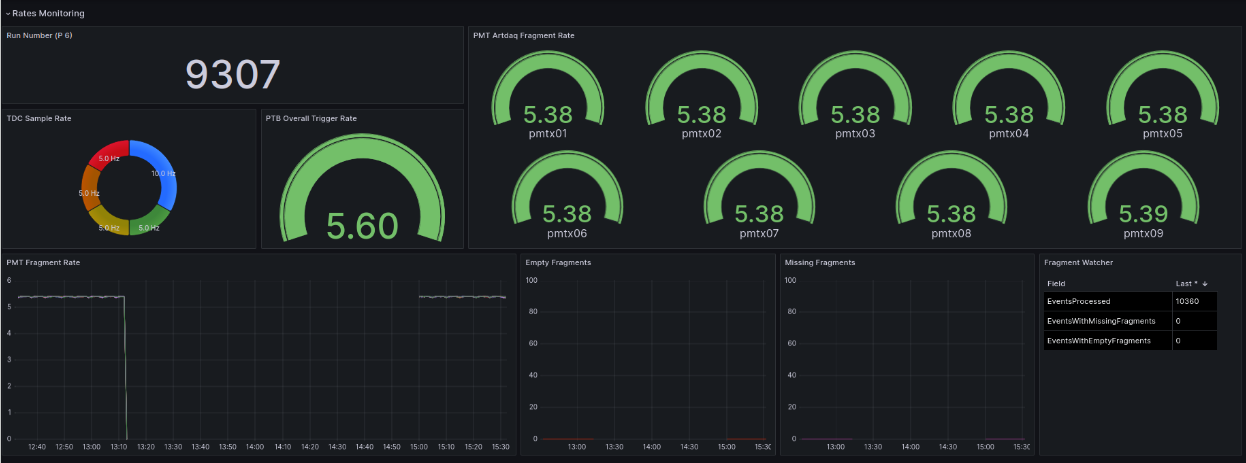
\includegraphics[width=1.0\textwidth]{Grafana}
\caption[Grafana Online Monitoring Web Page]{
Web page showing a section of Grafana for monitoring the status of PMT DAQ.
}
\label{fig:Grafana}
\vspace{0.5cm}
%\end{figure}
%\begin{figure}[htbp!] 
\centering    
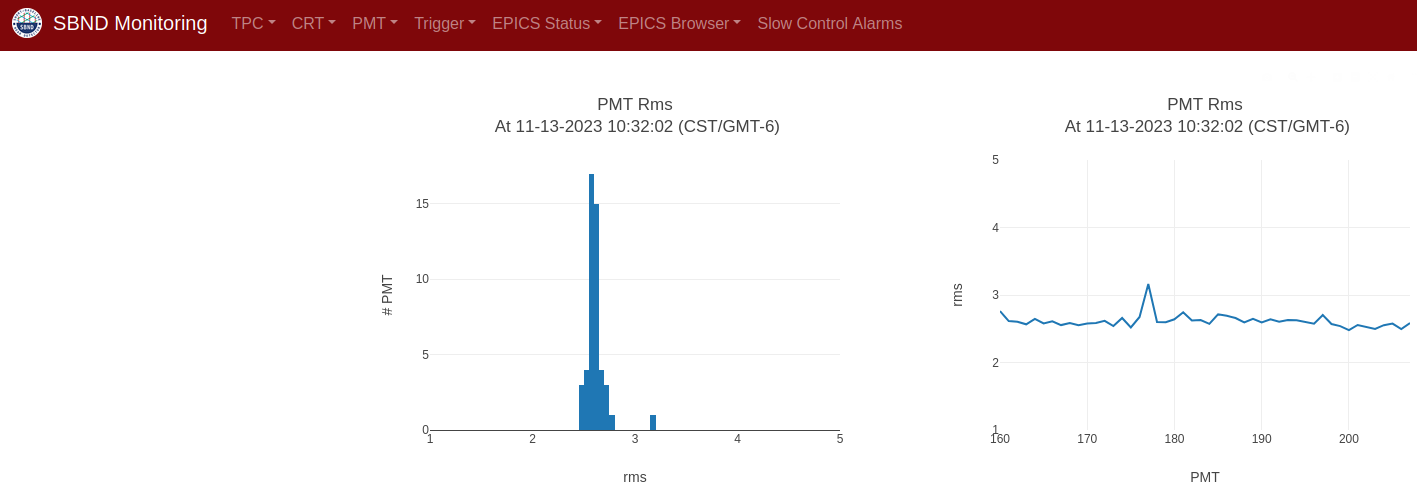
\includegraphics[width=1.0\textwidth]{Minargon}
\caption[Minargon Online Monitoring Web Page]{
Web page showing a section of Minargon for monitoring the root mean square of a PMT waveform baseline.
}
\label{fig:Minargon}
\end{figure}


